\begin{frame}
    \frametitle{Die Heuristik von Christofides - Schritt 1}
    Finde einen minimalen Spannbaum $T$ von $G$.
    \begin{itemize}
        \item bei uns: Kruskal-Algorithmus, $\mathcal{O}(|E|(|E|+|V|)) = \mathcal{O}(\frac{n(n-1)}{2}(\frac{n(n-1)}{2}+n)) = \mathcal{O}(n^4)$.
        \item in optimaler Implementierung mit Adjazenzmatrix: Prim $\mathcal{O}(|V|^2) = \mathcal{O}(n^2)$.
        \item $w(T) < w(H_{\mathrm{opt}})$ %add graphic
    \end{itemize}
    \only<2>{
		\begin{figure}
			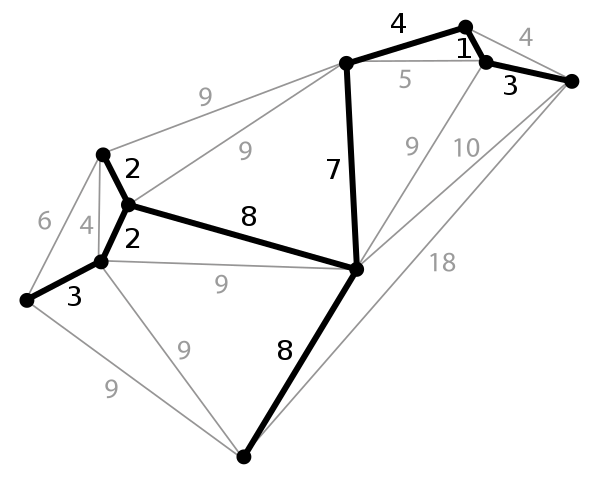
\includegraphics[scale=0.3]{images/tsp-msp}
			\caption{[Abb7] Traveling-Salesman-Problem}
		\end{figure}
	}
\end{frame}